\documentclass[10pt]{beamer}
\usefonttheme{serif}
\usetheme{Madrid}
% \usecolortheme{default}
\usecolortheme{beaver}
% \usecolortheme{crane}
\setbeamertemplate{navigation symbols}{}
\setbeamertemplate{footline}[frame number]

\usepackage{amsmath,amssymb,mathtools}


\title{Lab 2 Support Vector Machines}
\author{Lucas Frykman}
\date{February 18, 2026}
\begin{document}

% ────────────────────────────────────────────────
\begin{frame}
\titlepage
\end{frame}

% ────────────────────────────────────────────────
\begin{frame}{Key SVM Equations}
\small
\begin{itemize}
\item Primal (hard-margin): $\min \|{w}\| \quad$ s.t. $\quad t_i( {w}^\top{x}_i + b) \ge 1$
\item Soft-margin: \quad $\min \|{w}\| + C\sum\xi_i \quad$ s.t. $\quad t_i({w}^\top{x}_i + b) \ge 1-\xi_i, \ \xi_i\ge0$
\item Dual: \quad $\max_\alpha \sum \alpha_i - \frac{1}{2}\sum\alpha_i\alpha_j t_i t_j K({x}_i,{x}_j)$ s.t $0 \le \alpha_i \le C, \ \sum \alpha_i t_i = 0$
\item Indicator: $ \operatorname{ind}(s) = \operatorname{sgn}\Bigl( \sum_i \alpha_i t_i K({x}_i,{s}) + b \Bigr) \Leftrightarrow \operatorname{sgn} (w^T\cdot \phi(s) -b)$
\item Deicison boundary $s_0$ s.t $\sum_i \alpha_i t_i K({x}_i,{s_0}) + b = 0$
\end{itemize}
Kernels: Linear $K={x}^\top{y}$, Poly $(1+{x}^\top{y})^p$, RBF $\exp(-\|{x}-{y}\|^2/(2\sigma^2))$
\end{frame}


% ────────────────────────────────────────────────
\begin{frame}{Q1: Effect of Cluster Positions and Sizes}
\alert{Question:} Move clusters around/change sizes to make classification easier/harder. Note when optimizer fails.

\vspace{1em}

If clusters are far apart (e.g., class A at [1.5,0.5] \& [-1.5,0.5], class B at [0,-0.5], std=0.2): Easy separation, large margin, optimizer succeeds quickly.
As clusters move closer or increase spread (e.g., std=1.0, overlap): Harder, smaller margin.
If there's heavy overlap the optimizer fails for a sufficiently hard-margin / very small slack ('success'=False), as constraints can't be satisfied.

\vspace{1em}

Constraints $y_i({w}^\top {x}_i + b) \geq 1$ violated in overlap so no feasible solution exists
\end{frame}

\begin{frame}{Q1: Effect of Cluster Positions and Sizes}
    \centering
    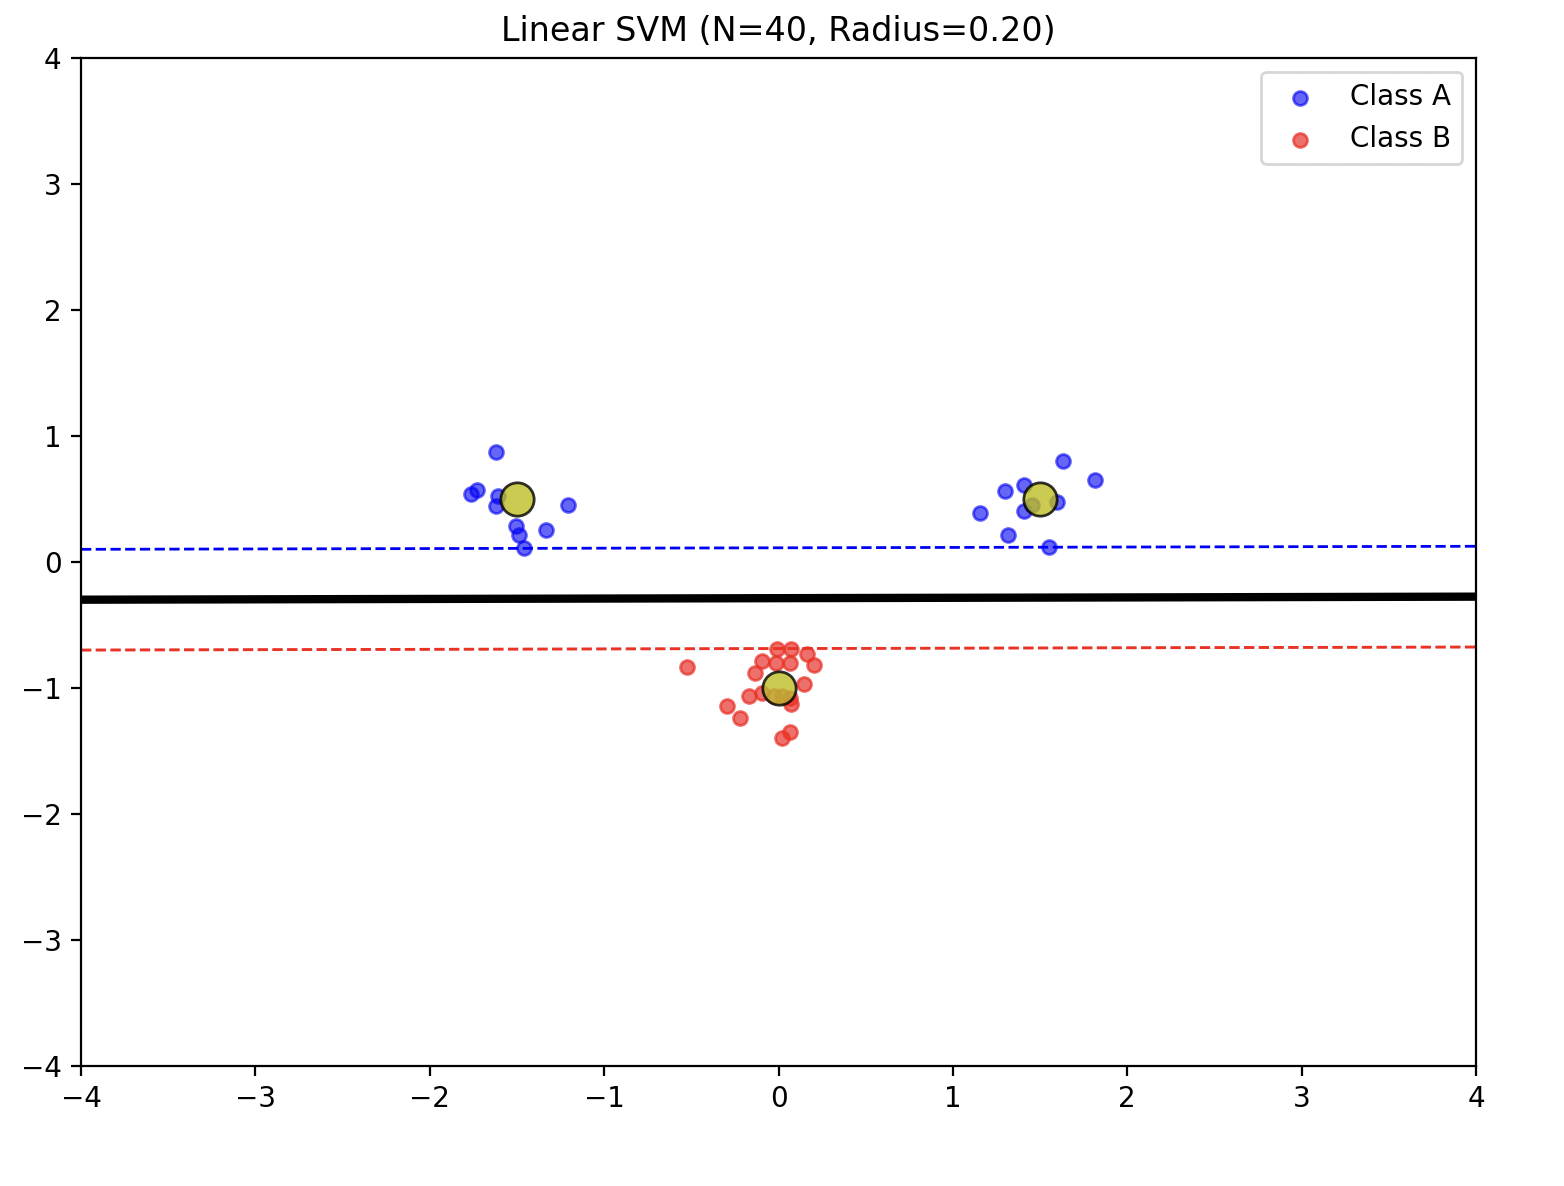
\includegraphics[width=0.8\textwidth]{image1.png}
\end{frame}
\begin{frame}{Q1: Effect of Cluster Positions and Sizes}
    \centering
    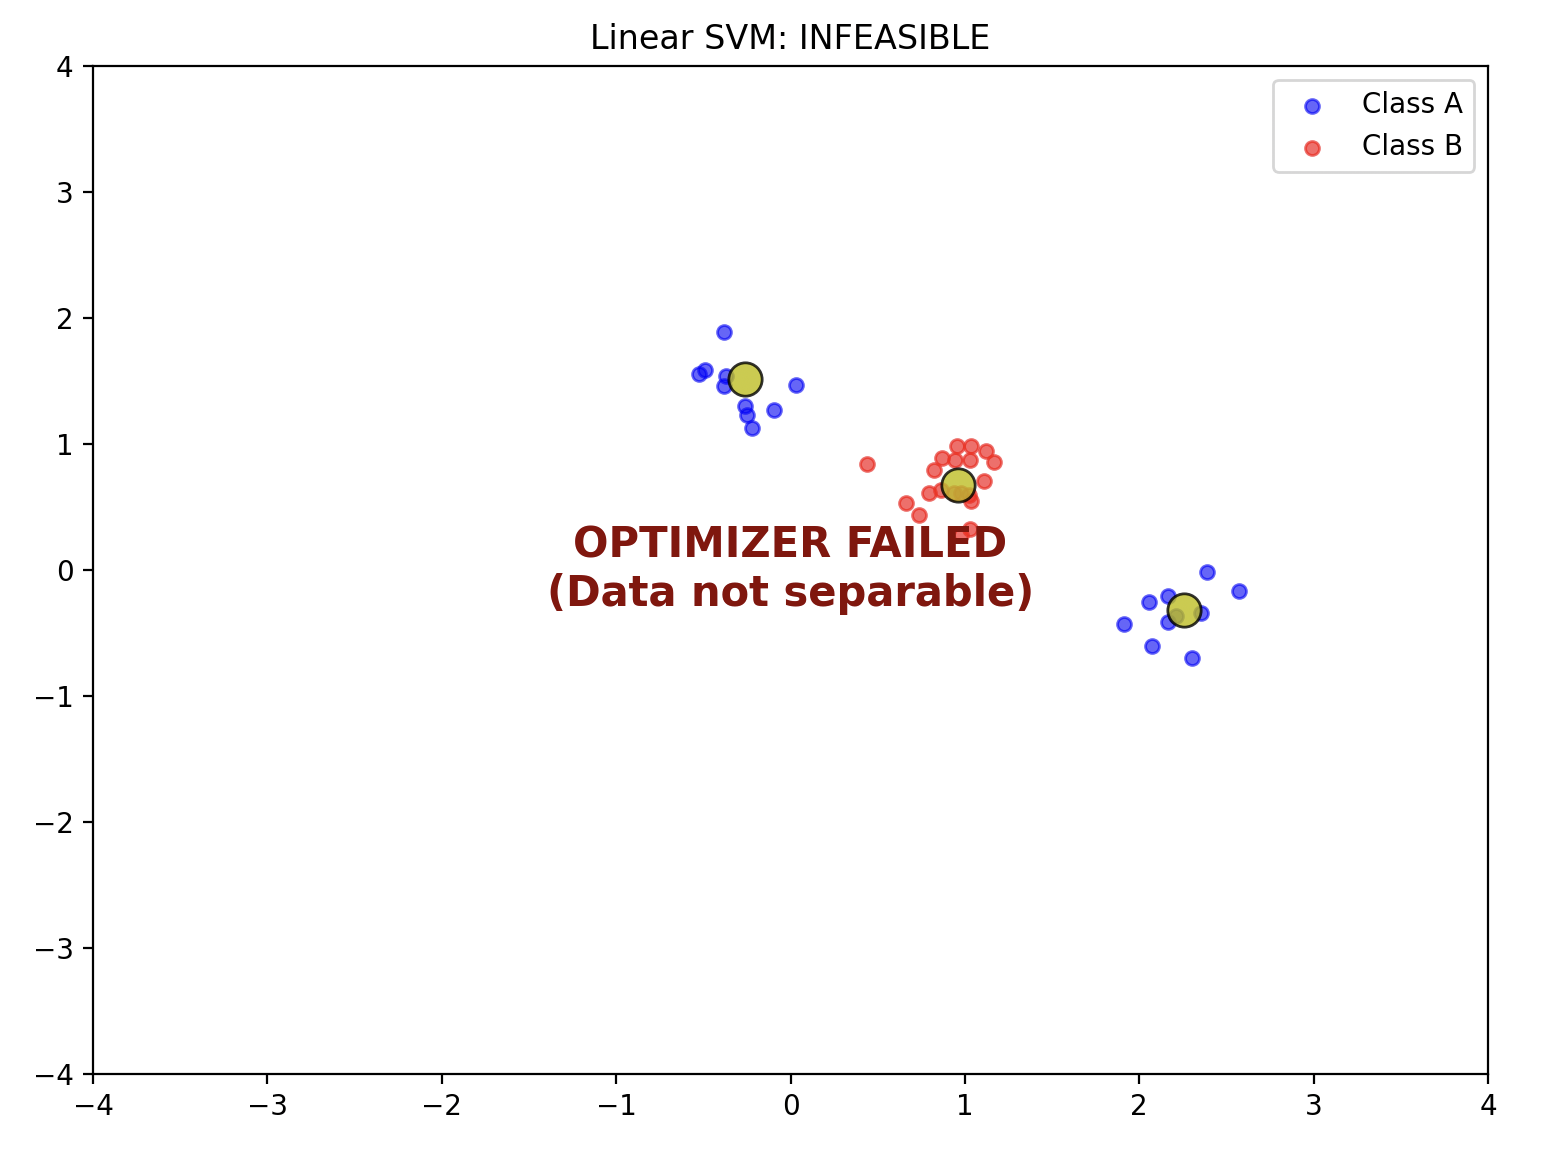
\includegraphics[width=0.8\textwidth]{image2.png}
\end{frame}
\begin{frame}{Q1: Effect of Cluster Positions and Sizes}
    \centering
    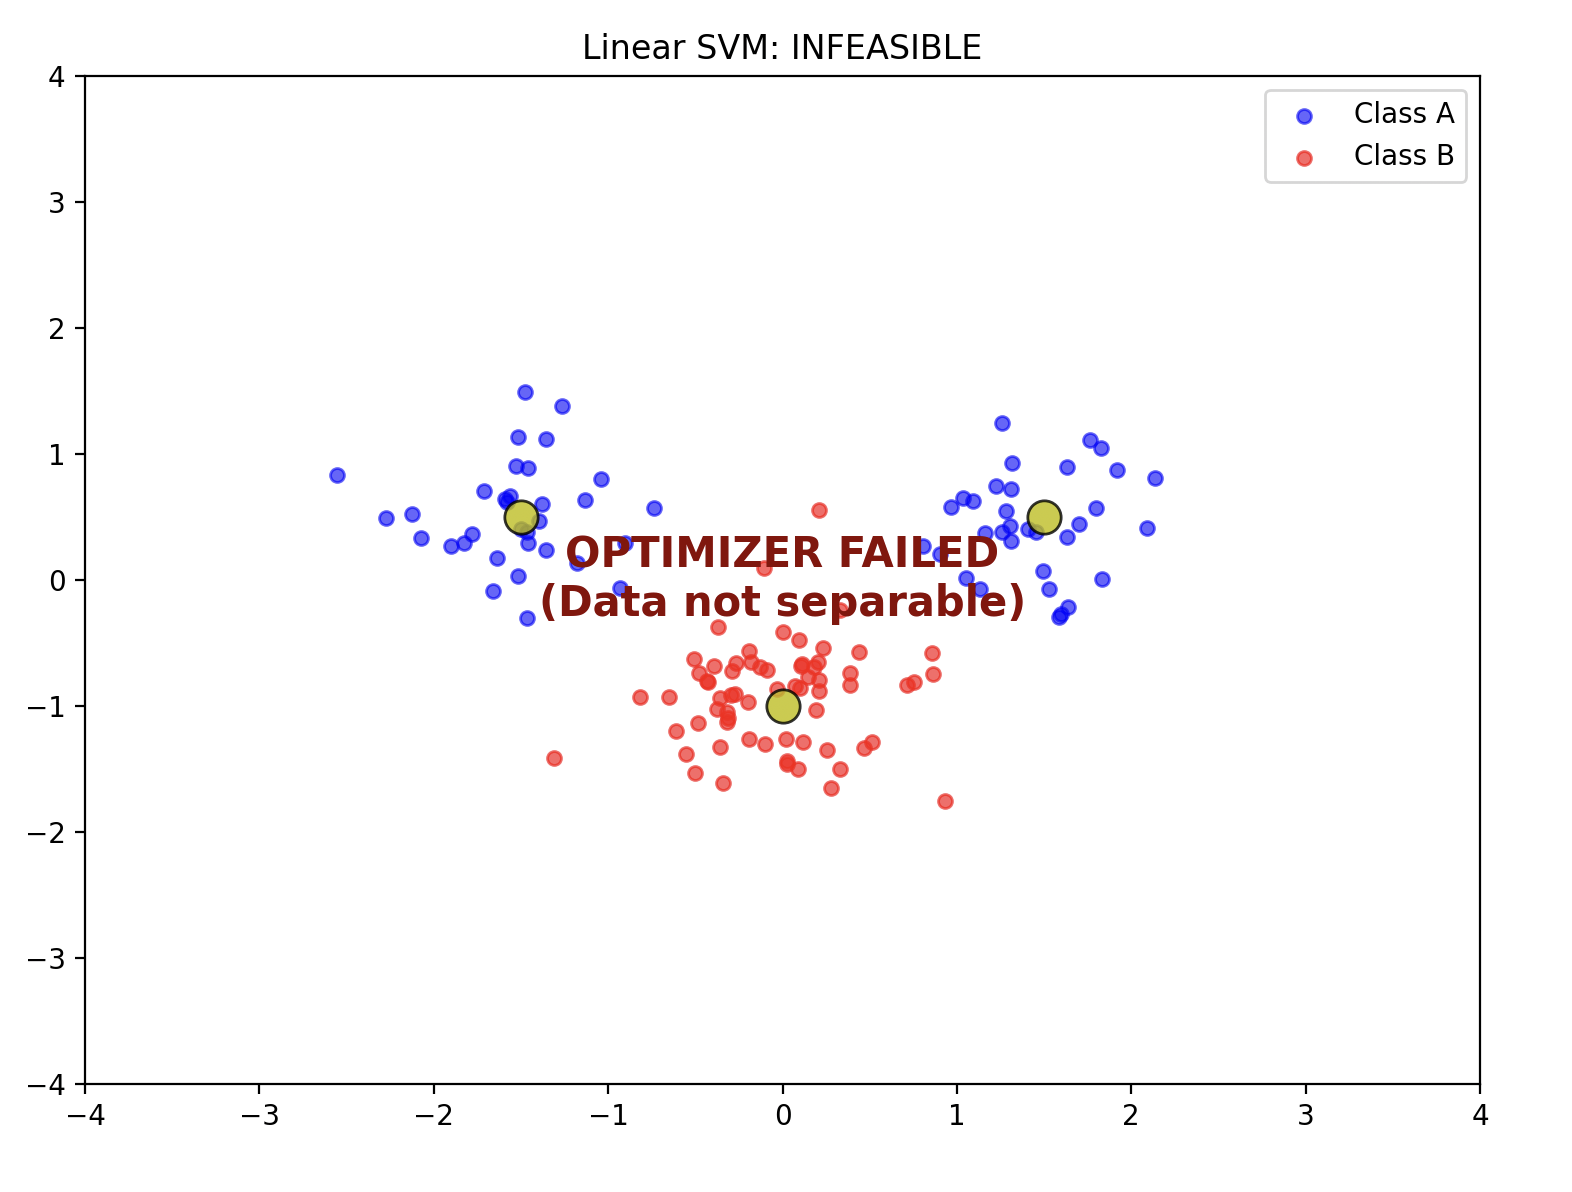
\includegraphics[width=0.8\textwidth]{image3.png}
\end{frame}
% ────────────────────────────────────────────────
% \begin{frame}{Q1: When Optimizer Fails}
% Without slack (hard-margin): If data not linearly separable, dual problem may not converge, minimize returns 'success': False. 
% Example: Overlapping clusters (class A/B centers close, high variance) $\to$ No hyperplane satisfies all constraints.
% Solution: Introduce slack (soft-margin) with $C > 0$, allowing violations via $\xi_i$.
%
% \vspace{1em}
%
% Soft-margin primal:
% \[
% \min \frac{1}{2}\|{w}\|^2 + C \sum \xi_i \quad \text{s.t.} \quad y_i({w}^\top {x}_i + b) \geq 1 - \xi_i, \ \xi_i \geq 0
% \]
%
% - Allows finding a solution even for hard cases.
% \end{frame}

% ────────────────────────────────────────────────
\begin{frame}{Q2: Implementing Non-Linear Kernels}
\alert{Question:} Implement polynomial and RBF kernels. Classify hard datasets.

\vspace{1em}

Linear kernel fails on non-linear data (e.g. circular clusters). \\
Polynomial: $K({x},{y}) = (1 + {x}^\top {y})^p$ $\to$ Curved boundaries (e:: p=2: quadratic). \\
RBF: $K({x},{y}) = \exp\left(-\frac{\|{x}-{y}\|^2}{2\sigma^2}\right)$ $\to$ Flexible, local boundaries.

\vspace{1em}

- For "very hard" datasets (e.g., moon-shaped or concentric circles): RBF can separate where linear/poly fail.
- Dual remains the same; just swap $K$ in objective: $\frac{1}{2} \sum_{i,j} \alpha_i \alpha_j t_i t_j K({x}_i, {x}_j) - \sum \alpha_i$
\end{frame}

% ────────────────────────────────────────────────
\begin{frame}{Q3: Kernel Parameters \& Bias-Variance Trade-off}
\alert{Question:} Explore how parameters influence boundary. Reason in bias-variance terms.

\vspace{1em}

Polynomial degree $p$: \\
- Low $p$ (e.g: 1=linear): High bias (underfit, simple boundary), low variance (stable). \\
- High $p$ (e.g: 7): Low bias (fits complex data), high variance (overfits noise, wiggly boundary). \\

RBF $\sigma$ (width): \\
- Large $\sigma$: Smooth boundary, high bias, low variance (underfit). \\
- Small $\sigma$: Jagged boundary, low bias, high variance (overfit, each point influences locally).

\vspace{1em}

\alert{Bias-Variance:} Complex params reduce bias but increase variance. Tune to balance (e.g., via cross-validation).
\end{frame}

\begin{frame}{Q3: Kernel Parameters \& Bias-Variance Trade-off}
\centering
    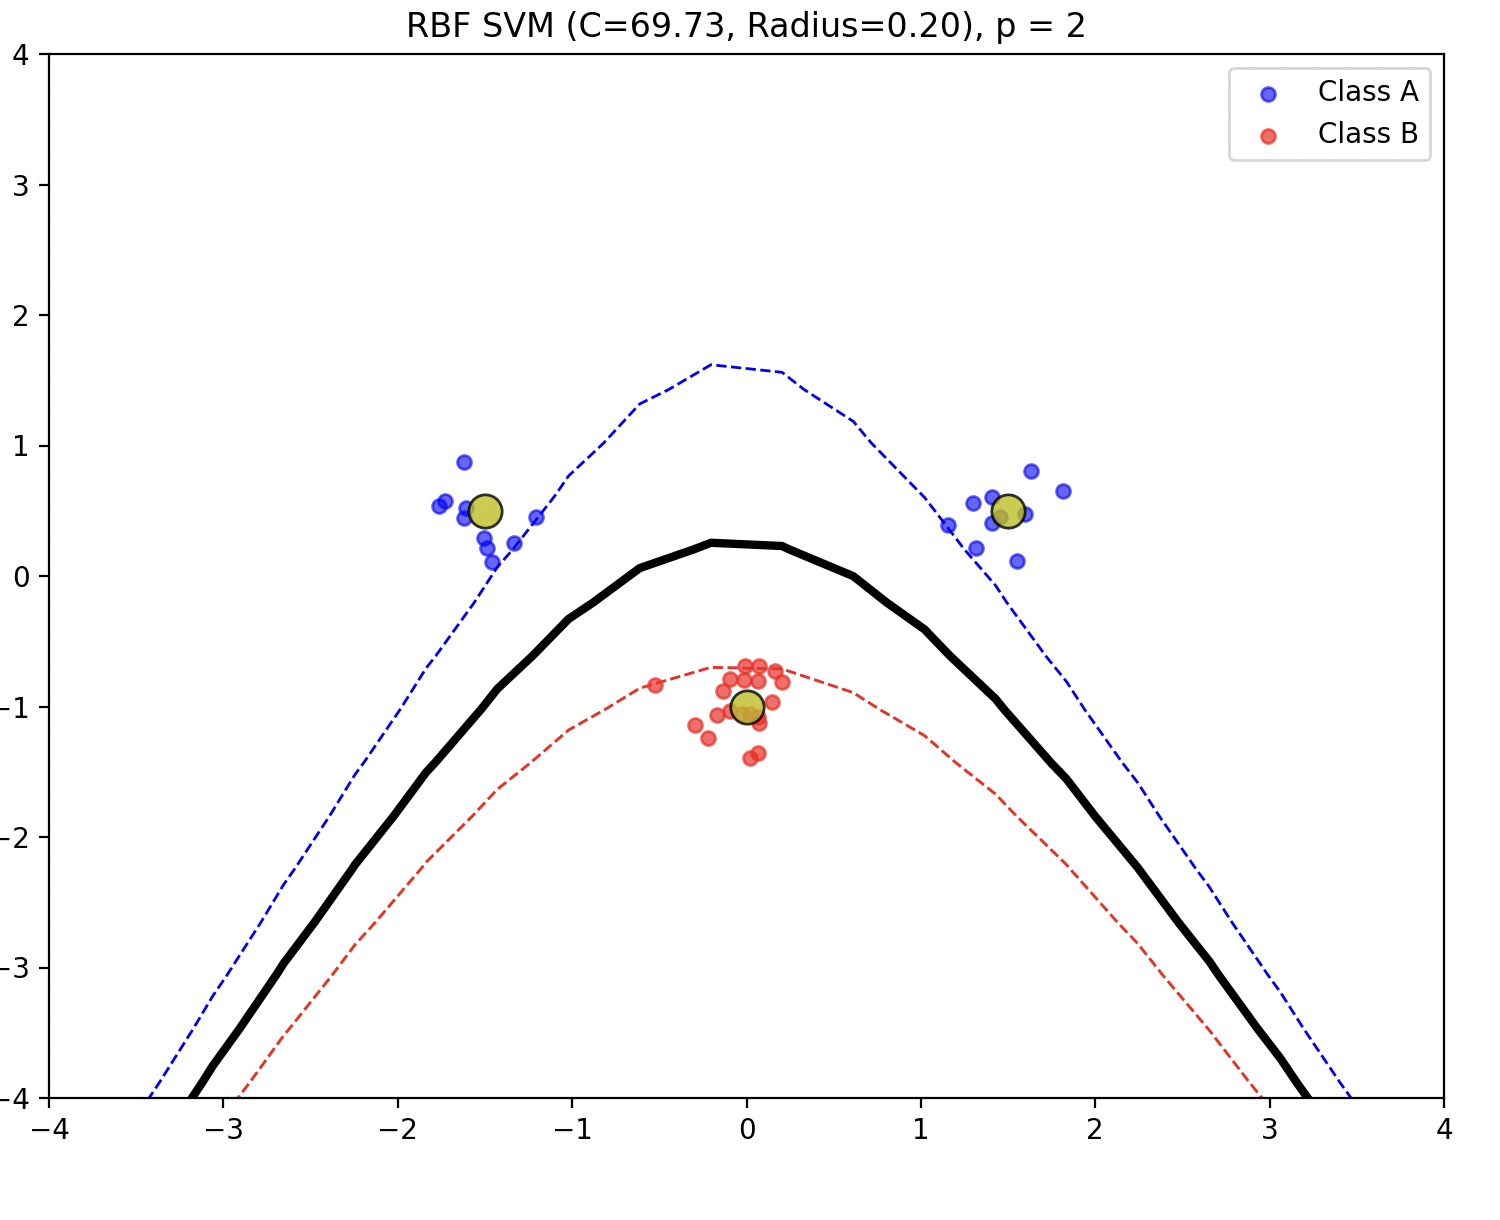
\includegraphics[width = 0.7\textwidth]{poly1}
\end{frame}
\begin{frame}{Q3: Kernel Parameters \& Bias-Variance Trade-off}
\centering
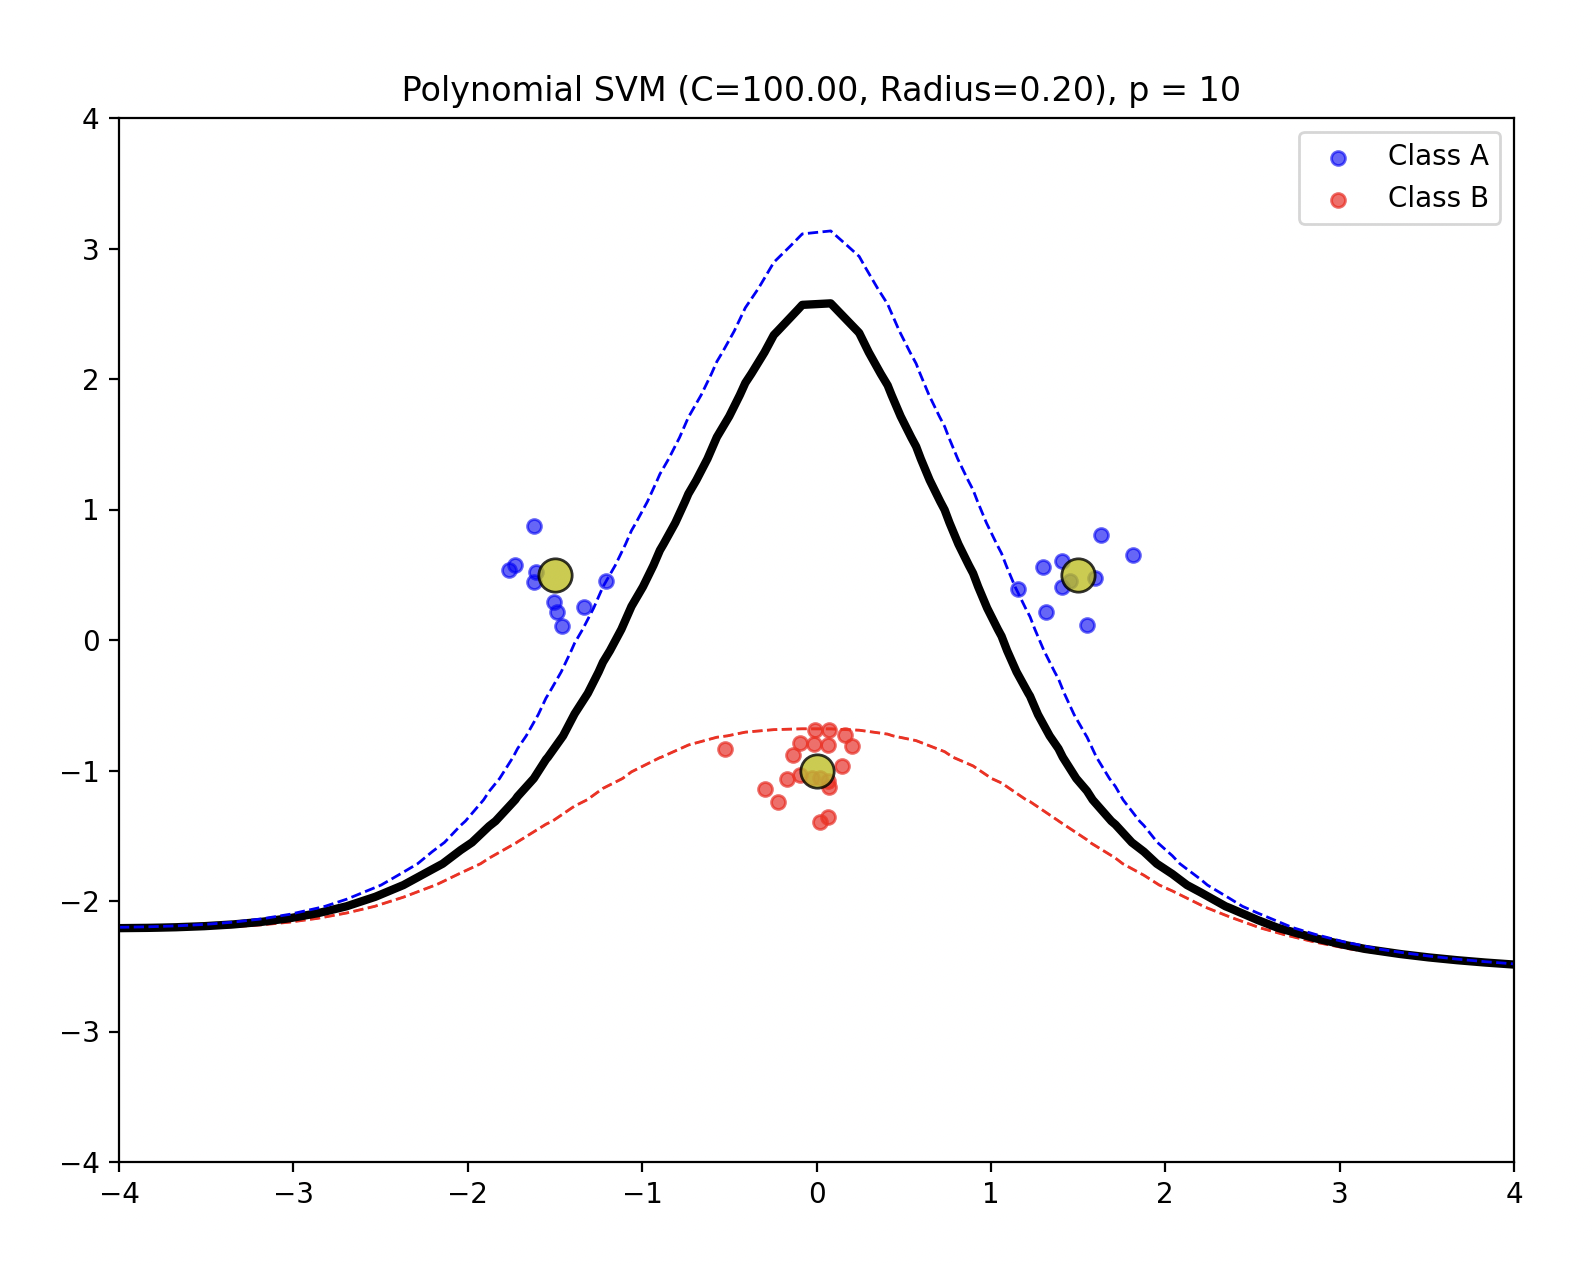
\includegraphics[width = 0.7\textwidth]{poly2}
\end{frame}
\begin{frame}{Q3: Kernel Parameters \& Bias-Variance Trade-off}
\centering
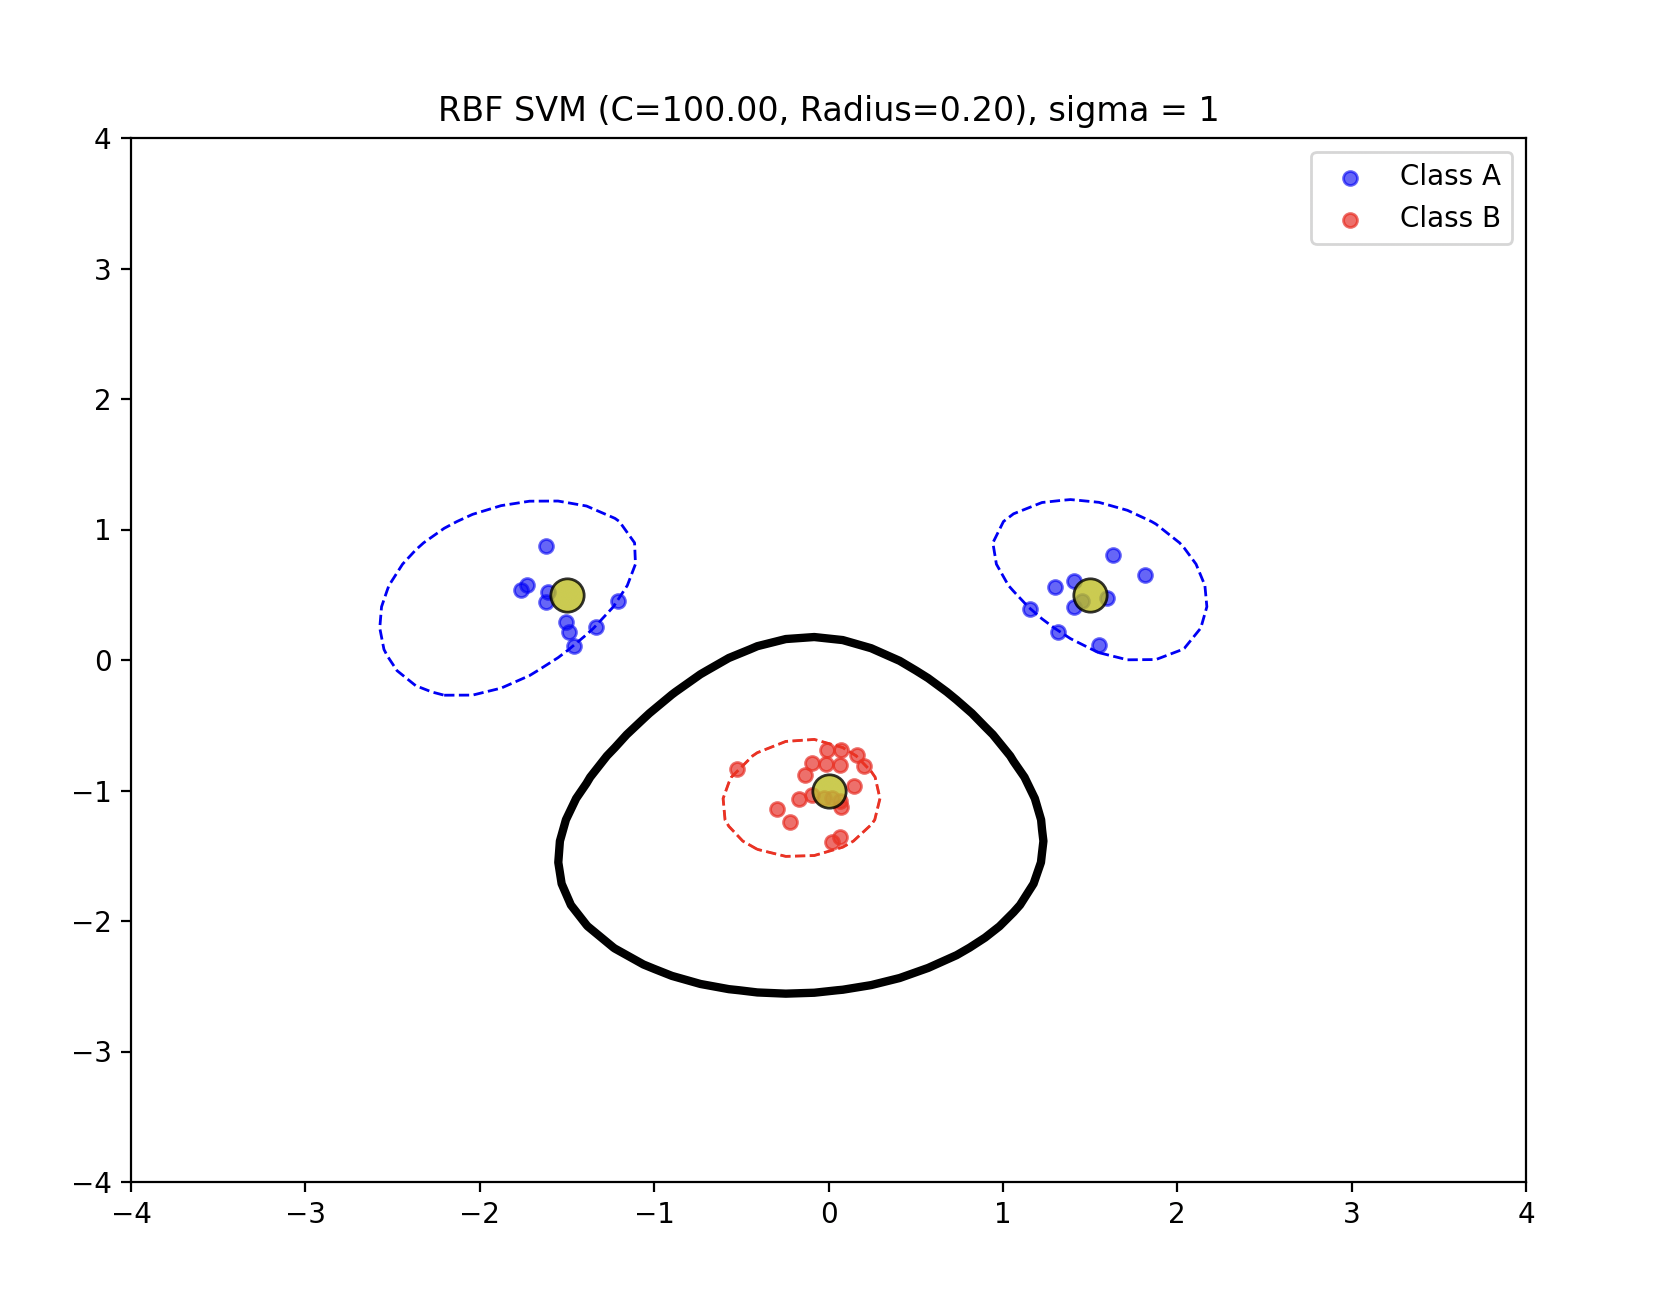
\includegraphics[width = 0.7\textwidth]{sigma1}
\end{frame}
\begin{frame}{Q3: Kernel Parameters \& Bias-Variance Trade-off}
\centering
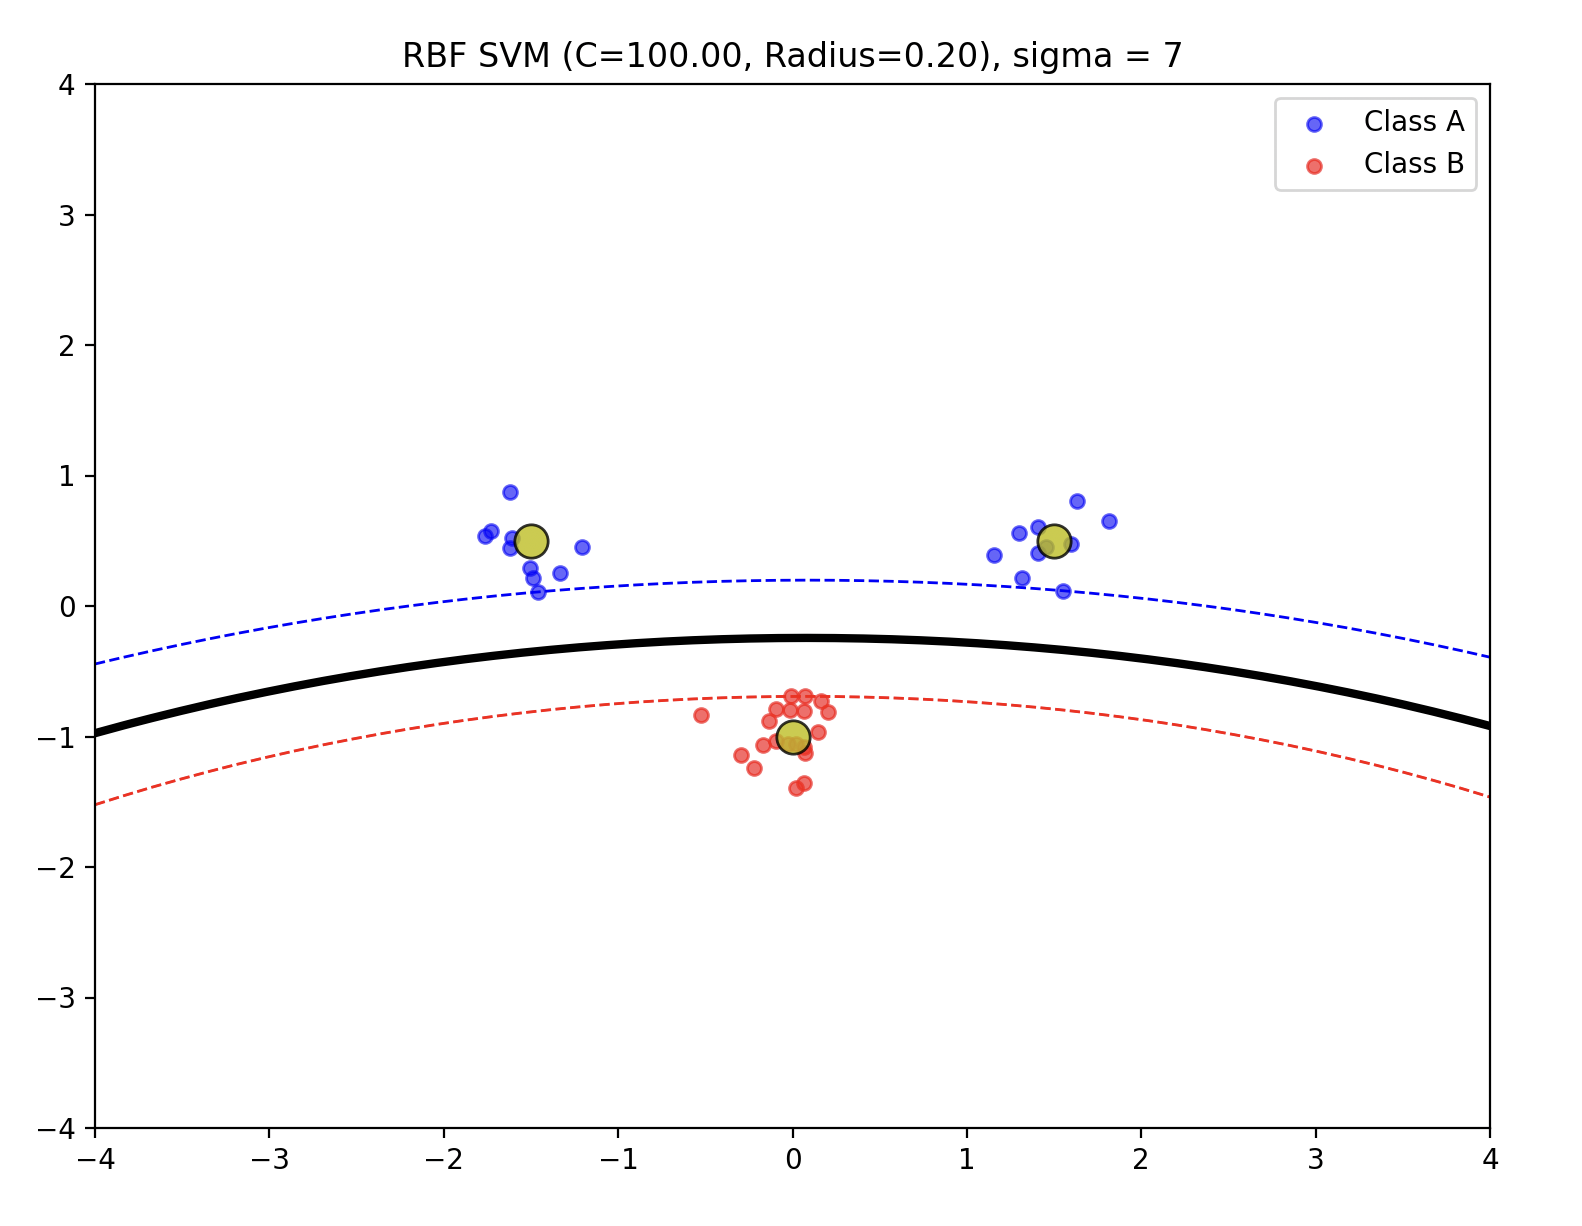
\includegraphics[width = 0.7\textwidth]{sigma2}
\end{frame}
% ────────────────────────────────────────────────
\begin{frame}{Q4: Role of Slack Parameter $C$}
\alert{Question:} Explore $C$; what for large/small values?

\vspace{1em}

$C$ controls trade-off: Margin width vs. misclassifications. \\
Large $C$ (e.g: $100$): Heavy penalty on $\xi_i$ allows for almost no missclassifications of training data, small margin, potential overfit (low bias, high variance). The resulting thinner margin means
the boundary decision will be more sensitive to the training data.\\
Small $C$ (e.g: $0.1$): Lighter penalty allows for more missclassifications of training data, larger margin, underfit if too small (high bias, low variance). The resulting thicker margin means the boundary decision
means the boundary decision will be less sensitive to the training data and might generalize better.

\vspace{1em}

Soft-margin objective function:
\[
\min \frac{1}{2}\|{w}\|^2 + C \sum \xi_i
\]

% - Noisy data: Small $C$ ignores outliers. \\
% - Clean data: Large $C$ enforces hard-margin-like behavior.
\end{frame}

\begin{frame}{Q4: Role of Slack Parameter $C$}

\centering
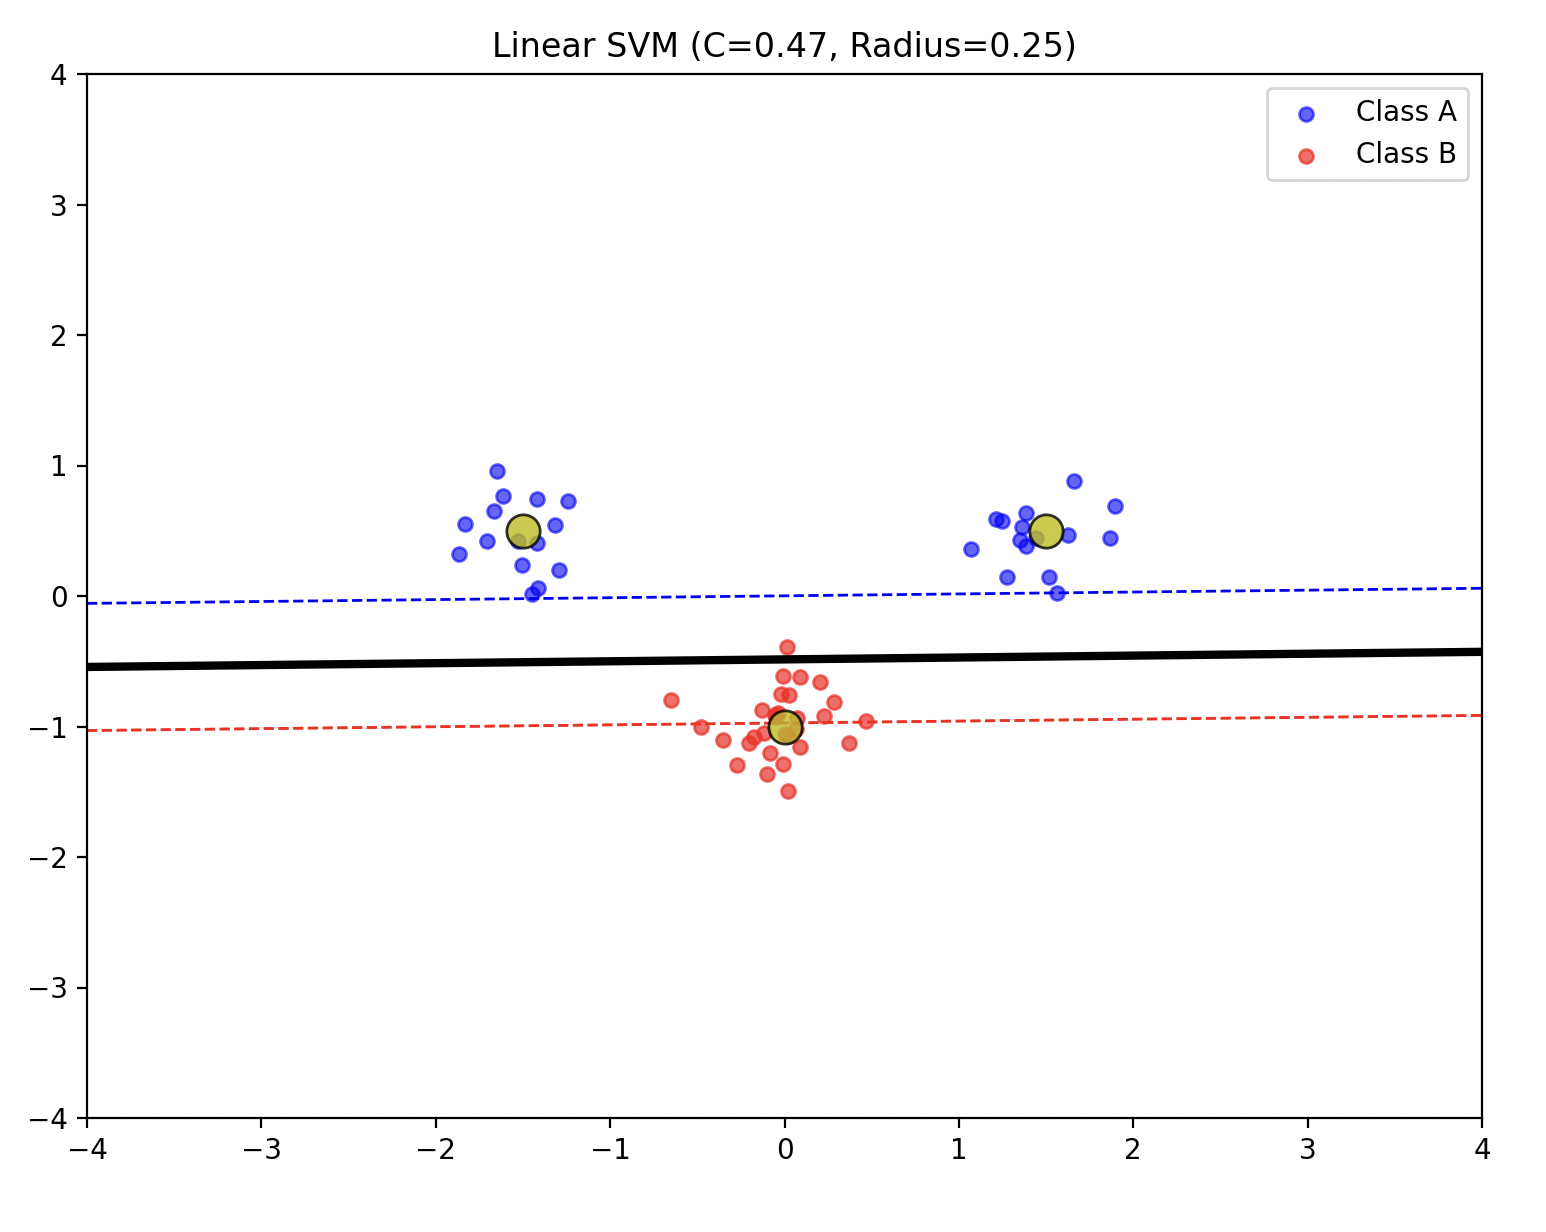
\includegraphics[width = 0.7\textwidth]{bigC}
\end{frame}
\begin{frame}{Q4: Role of Slack Parameter $C$}
\centering
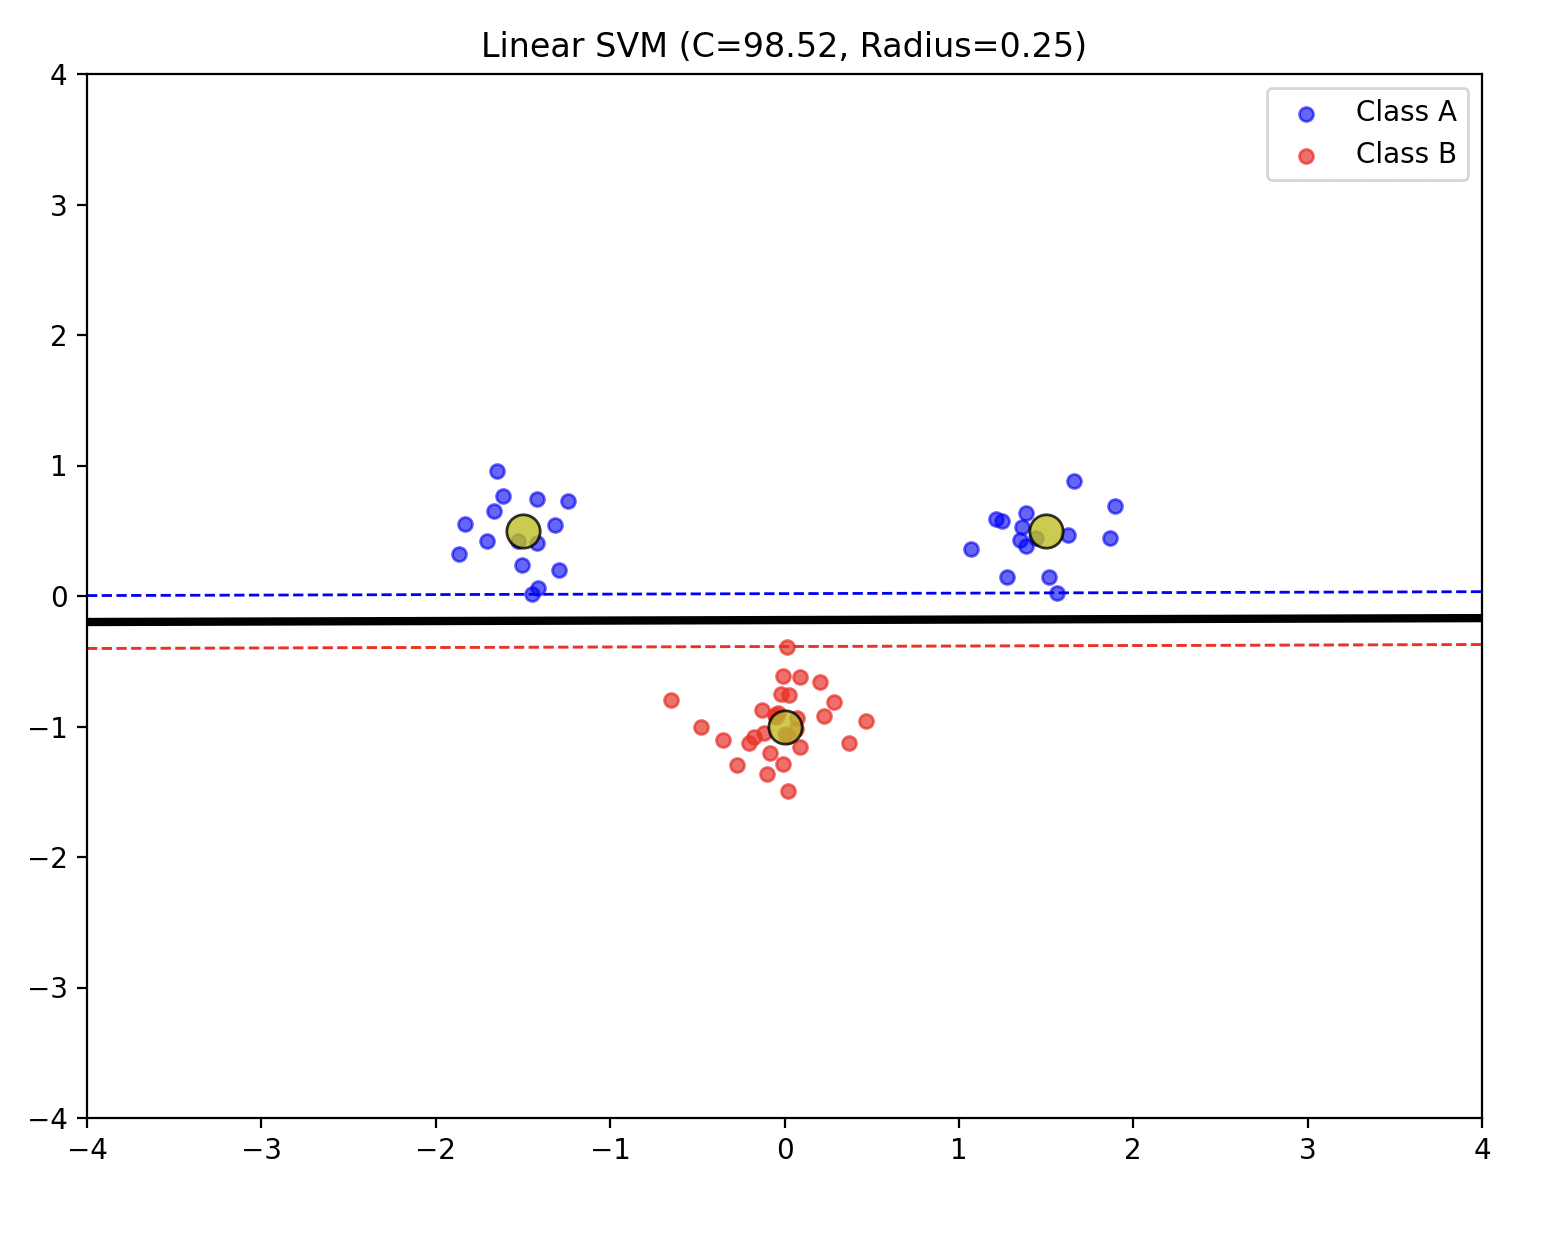
\includegraphics[width = 0.7\textwidth]{smallC}
\end{frame}
% ────────────────────────────────────────────────
\begin{frame}{Q5: Slack vs. Complex Model for Non-Separable Data}
\alert{Question:} When opt for more slack vs. more complex kernel?

\vspace{1em}

\alert{More slack (small $C$):} When you have low training error relative to test error. Normally indicative that data has noise. Allows ignoring anomalies for larger margin, avoids overfit. Prefer when true boundary is simple but data noisy. 
\alert{More complex kernel (e.g: high $p$ poly or small $\sigma$ RBF):} If data inherently non-linear/complex. Captures true patterns, but risk overfit if noise present. When both your training error
and test error is too high.

% \vspace{1em}
%
% - Rule: If adding complexity improves validation but not training complex kernel.
% - If data noisy (high variance): Increase slack first.
% - Balance: Use CV to compare (e.g., small $C$ + linear vs. large $C$ + RBF).
\end{frame}

% ────────────────────────────────────────────────
% \begin{frame}{Summary}
% These slides address the lab's exploration questions using SVM equations and reasoning.
% - Q1-Q2: Data separability \& kernels.
% - Q3-Q4: Parameters for regularization.
% - Q5: Practical trade-offs.
%
% For plots: Generate in code (e.g., vary clusters/C/params) and observe boundaries/margins/SVs.
% \end{frame}

\end{document}
